\documentclass{beamer}

\pdfmapfile{+sansmathaccent.map}


\mode<presentation>
{
	\usetheme{Warsaw} % or try Darmstadt, Madrid, Warsaw, Rochester, CambridgeUS, ...
	\usecolortheme{seahorse} % or try seahorse, beaver, crane, wolverine, ...
	\usefonttheme{serif}  % or try serif, structurebold, ...
	\setbeamertemplate{navigation symbols}{}
	\setbeamertemplate{caption}[numbered]
} 


%%%%%%%%%%%%%%%%%%%%%%%%%%%%
% itemize settings


%%%%%%%%%%%%%%%%%%%%%%%%%%%%
% itemize settings

\definecolor{myhotpink}{RGB}{255, 80, 200}
\definecolor{mywarmpink}{RGB}{255, 60, 160}
\definecolor{mylightpink}{RGB}{255, 80, 200}
\definecolor{mypink}{RGB}{255, 30, 80}
\definecolor{mydarkpink}{RGB}{155, 25, 60}

\definecolor{mypaleblue}{RGB}{240, 240, 255}
\definecolor{mylightblue}{RGB}{120, 150, 255}
\definecolor{myblue}{RGB}{90, 90, 255}
\definecolor{mygblue}{RGB}{70, 110, 240}
\definecolor{mydarkblue}{RGB}{0, 0, 180}
\definecolor{myblackblue}{RGB}{40, 40, 120}

\definecolor{myblackturquoise}{RGB}{5, 53, 60}
\definecolor{mydarkdarkturquoise}{RGB}{8, 93, 110}
\definecolor{mydarkturquoise}{RGB}{28, 143, 150}
\definecolor{mypaleturquoise}{RGB}{230, 255, 255}
\definecolor{myturquoise}{RGB}{48, 213, 200}

\definecolor{mygreen}{RGB}{0, 200, 0}
\definecolor{mydarkgreen}{RGB}{0, 120, 0}
\definecolor{mygreen2}{RGB}{245, 255, 230}

\definecolor{mygrey}{RGB}{120, 120, 120}
\definecolor{mypalegrey}{RGB}{160, 160, 160}
\definecolor{mydarkgrey}{RGB}{80, 80, 160}

\definecolor{mydarkred}{RGB}{160, 30, 30}
\definecolor{mylightred}{RGB}{255, 150, 150}
\definecolor{myred}{RGB}{200, 110, 110}
\definecolor{myblackred}{RGB}{120, 40, 40}

\definecolor{mygreen}{RGB}{0, 200, 0}
\definecolor{mygreen2}{RGB}{205, 255, 200}

\definecolor{mydarkcolor}{RGB}{60, 25, 155}
\definecolor{mylightcolor}{RGB}{130, 180, 250}

\setbeamertemplate{itemize items}[default]

\setbeamertemplate{itemize item}{\color{myblackturquoise}$\blacksquare$}
\setbeamertemplate{itemize subitem}{\color{mydarkdarkturquoise}$\blacktriangleright$}
\setbeamertemplate{itemize subsubitem}{\color{mygray}$\blacksquare$}

\setbeamercolor{palette quaternary}{fg=white,bg=myblackturquoise}
\setbeamercolor{titlelike}{parent=palette quaternary}

\setbeamercolor{palette quaternary2}{fg=black,bg=mypaleblue}
\setbeamercolor{frametitle}{parent=palette quaternary2}

\setbeamerfont{frametitle}{size=\Large,series=\scshape}
\setbeamerfont{framesubtitle}{size=\normalsize,series=\upshape}





%%%%%%%%%%%%%%%%%%%%%%%%%%%%
% block settings

\setbeamercolor{block title}{bg=red!30,fg=black}

\setbeamercolor*{block title example}{bg=mygreen!40!white,fg=black}

\setbeamercolor*{block body example}{fg= black, bg= mygreen2}


%%%%%%%%%%%%%%%%%%%%%%%%%%%%
% URL settings
\hypersetup{
	colorlinks=true,
	linkcolor=blue,
	filecolor=blue,      
	urlcolor=blue,
}

%%%%%%%%%%%%%%%%%%%%%%%%%%

\renewcommand{\familydefault}{\rmdefault}

\usepackage{amsmath}
\usepackage{mathtools}

\usepackage{subcaption}

\usepackage{qrcode}

\DeclareMathOperator*{\argmin}{arg\,min}
\newcommand{\bo}[1] {\mathbf{#1}}

\newcommand{\R}{\mathbb{R}} 
\newcommand{\T}{^\top}     



\newcommand{\mydate}{Fall 2023}

\newcommand{\mygit}{\textcolor{blue}{\href{https://github.com/SergeiSa/Control-Theory-Slides-Spring-2023}{github.com/SergeiSa/Control-Theory-Slides-Spring-2023}}}

\newcommand{\myqr}{ \textcolor{black}{\qrcode[height=1.5in]{https://github.com/SergeiSa/Control-Theory-Slides-Spring-2023}}
}

\newcommand{\myqrframe}{
	\begin{frame}
		\centerline{Lecture slides are available via Github, links are on Moodle}
		\bigskip
		\centerline{You can help improve these slides at:}
		\centerline{\mygit}
		\bigskip
		\myqr
	\end{frame}
}


\newcommand{\bref}[2] {\textcolor{blue}{\href{#1}{#2}}}

%%%%%%%%%%%%%%%%%%%%%%%%%%%%
% code settings

\usepackage{listings}
\usepackage{color}
% \definecolor{mygreen}{rgb}{0,0.6,0}
% \definecolor{mygray}{rgb}{0.5,0.5,0.5}
\definecolor{mymauve}{rgb}{0.58,0,0.82}
\lstset{ 
	backgroundcolor=\color{white},   % choose the background color; you must add \usepackage{color} or \usepackage{xcolor}; should come as last argument
	basicstyle=\footnotesize,        % the size of the fonts that are used for the code
	breakatwhitespace=false,         % sets if automatic breaks should only happen at whitespace
	breaklines=true,                 % sets automatic line breaking
	captionpos=b,                    % sets the caption-position to bottom
	commentstyle=\color{mygreen},    % comment style
	deletekeywords={...},            % if you want to delete keywords from the given language
	escapeinside={\%*}{*)},          % if you want to add LaTeX within your code
	extendedchars=true,              % lets you use non-ASCII characters; for 8-bits encodings only, does not work with UTF-8
	firstnumber=0000,                % start line enumeration with line 0000
	frame=single,	                   % adds a frame around the code
	keepspaces=true,                 % keeps spaces in text, useful for keeping indentation of code (possibly needs columns=flexible)
	keywordstyle=\color{blue},       % keyword style
	language=Octave,                 % the language of the code
	morekeywords={*,...},            % if you want to add more keywords to the set
	numbers=left,                    % where to put the line-numbers; possible values are (none, left, right)
	numbersep=5pt,                   % how far the line-numbers are from the code
	numberstyle=\tiny\color{mygray}, % the style that is used for the line-numbers
	rulecolor=\color{black},         % if not set, the frame-color may be changed on line-breaks within not-black text (e.g. comments (green here))
	showspaces=false,                % show spaces everywhere adding particular underscores; it overrides 'showstringspaces'
	showstringspaces=false,          % underline spaces within strings only
	showtabs=false,                  % show tabs within strings adding particular underscores
	stepnumber=2,                    % the step between two line-numbers. If it's 1, each line will be numbered
	stringstyle=\color{mymauve},     % string literal style
	tabsize=2,	                   % sets default tabsize to 2 spaces
	title=\lstname                   % show the filename of files included with \lstinputlisting; also try caption instead of title
}


%%%%%%%%%%%%%%%%%%%%%%%%%%%%
% URL settings
\hypersetup{
	colorlinks=false,
	linkcolor=blue,
	filecolor=blue,      
	urlcolor=blue,
}

%%%%%%%%%%%%%%%%%%%%%%%%%%

%%%%%%%%%%%%%%%%%%%%%%%%%%%%
% tikz settings

\usepackage{tikz}
\tikzset{every picture/.style={line width=0.75pt}}


\title{Optical sensors}
\subtitle{Mechatronics, Lecture 9}
\author{by Sergei Savin}
\centering
\date{\mydate}



\begin{document}
\maketitle



\begin{frame}{Content}
\begin{itemize}
	\item Measuring rotation
	\item Optical encoder
	\item Direction of rotation
	\item Relative vs absolute encoders
	\item Binary vs gray code
	\item Placement of optical sensors
\end{itemize}
\end{frame}




\begin{frame}{Measuring rotation}
	% \framesubtitle{O}
	\begin{flushleft}
		
		Rotation can be measured in many possible ways. Among them:
		
		\begin{itemize}
			\item measuring 1D rotation with optical encoder;
			\item measuring 1D rotation with hall effect encoder;
			\item measuring 3D orientation with IMU.
		\end{itemize}
		
		
	\end{flushleft}
\end{frame}



\begin{frame}{Optical encoder}
	% \framesubtitle{O}
	\begin{flushleft}
		
		Optical encoders are characterized by the use of sources of light passing through disk with openings spaced at regular intervals:
		
		% TODO: \usepackage{graphicx} required
		\begin{figure}
			\centering
			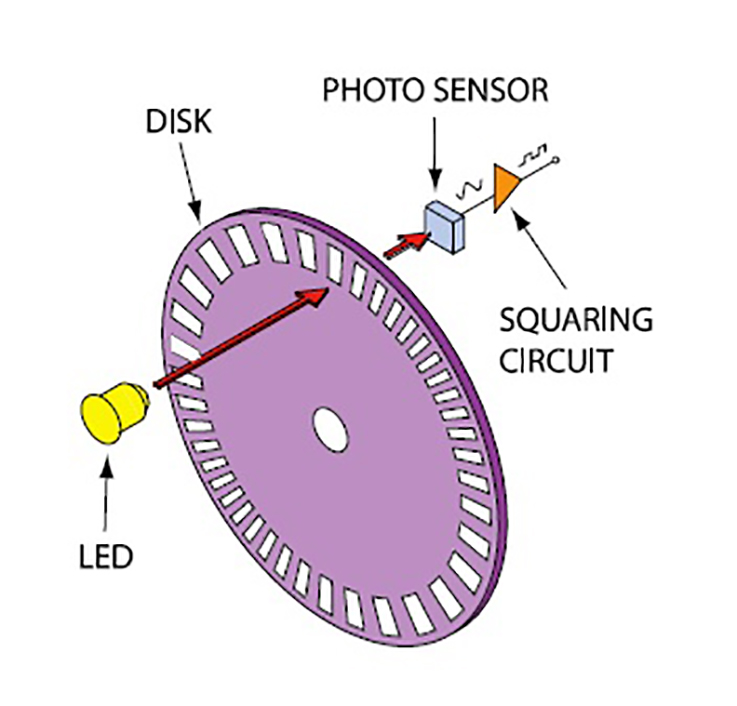
\includegraphics[width=0.5\linewidth]{encoder1}
			\caption{Optical encoder}
			\label{fig:encoder1}
		\end{figure}
		
		
	\end{flushleft}
\end{frame}



\begin{frame}{Optical encoder - working principle}
	% \framesubtitle{O}
	\begin{flushleft}
		
		Disk of the optical encoder is attached to the motor shaft, which rotation is measured. 
		
		\bigskip
		
		While the shaft and the disk are rotating, the light from the light source is being periodically blocked. The photo sensor is producing voltage as a function of the strength of the light that reaches the sensor. This results in a square waveform.
		
		\bigskip
		
		Counting how many times the voltage goes from high to low per unit of time, we can estimate angular velocity of the shaft.
		
	\end{flushleft}
\end{frame}



\begin{frame}{Direction of rotation}
	% \framesubtitle{O}
	\begin{flushleft}
		
		Direction of rotation is estimated using \emph{quadrature} encoder. It is achieved by placing two sensors with an offset (in terms of phase) allowing to compare their reading. When sensor A detects a change from high to low ahead of the sensor B - it encodes one direction of rotation,.e.g. clockwise. When sensor B is reading the change ahead of the sensor A - it encodes the opposite direction of rotation,.e.g. counter-clockwise:
		
		% TODO: \usepackage{graphicx} required
		\begin{figure}
			\centering
			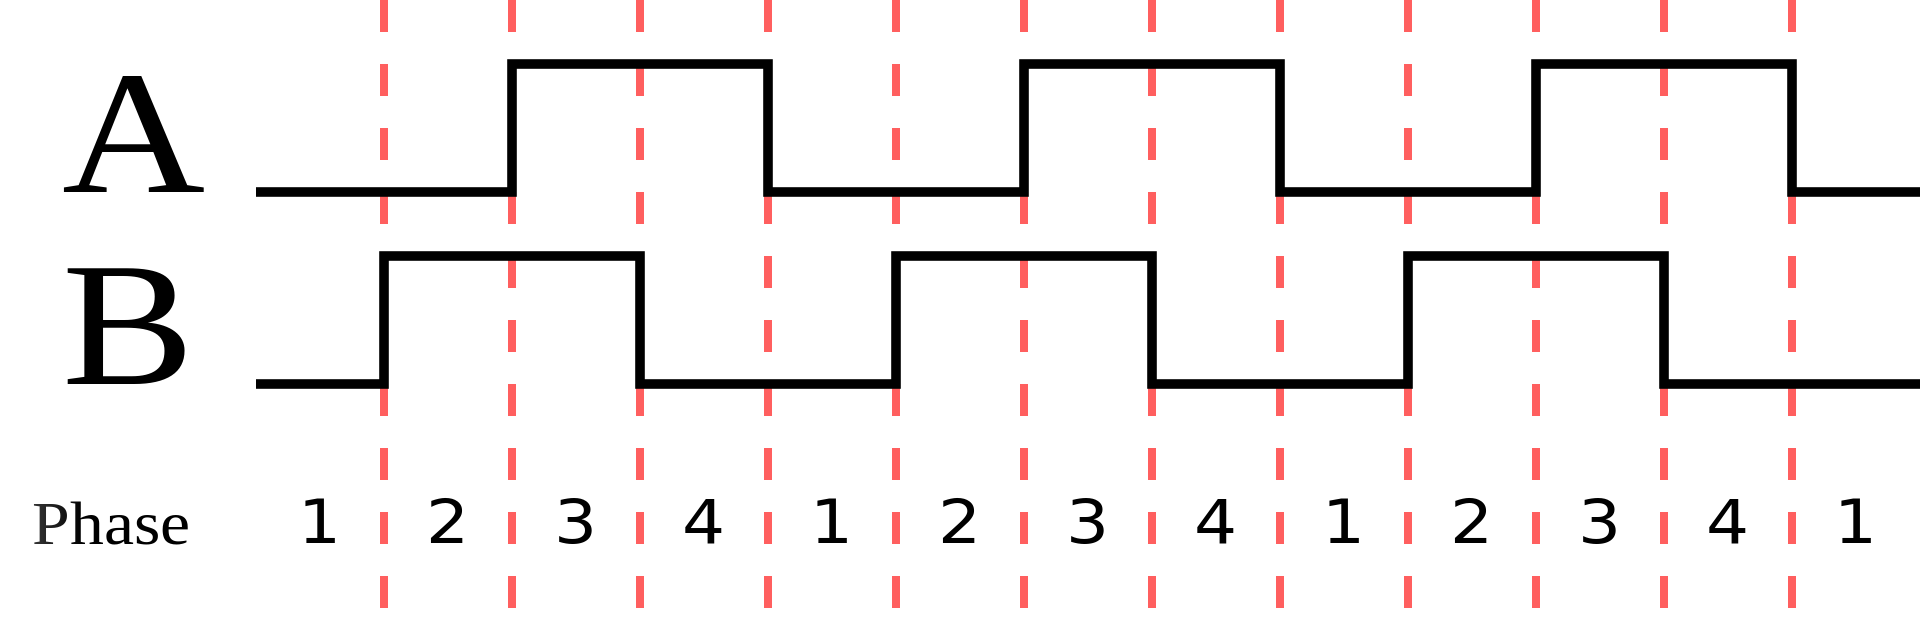
\includegraphics[width=0.7\linewidth]{Quadrature_Diagram.svg}
%			\caption{}
			\label{fig:quadraturediagram}
		\end{figure}
		
		
	\end{flushleft}
\end{frame}



\begin{frame}{Orientation vs velocity}
	% \framesubtitle{O}
	\begin{flushleft}
		
		As mentioned before, we can estimate velocity as the number of voltage changes per unit of time. 
		
		\bigskip
		
		To estimate the angle of rotation we can multiply velocity by the time - or more directly, by counting number of voltage changes, taking into account direction of rotation. However, in case the direction of rotation changes often and fast, it is possible to accrue estimation error.
		
		
	\end{flushleft}
\end{frame}


\begin{frame}{Incremental vs absolute encoders}
	% \framesubtitle{O}
	\begin{flushleft}
		
		Incremental (relative) encoders are defined by inability to detect initial orientation of the shaft. Instead, they are only able to measure change on the orientation relative to the initial position of the shaft. The encoders we have looked at so far are incremental.
		
		\bigskip
		
		Absolute encoders are are able to measure initial orientation of the shaft. In optical encoders, it is done by placing multiple light sensors and encoding each possible orientation with a certain code.
		
	\end{flushleft}
\end{frame}




\begin{frame}{Absolute encoder}
	% \framesubtitle{O}
	\begin{flushleft}
		
		% TODO: \usepackage{graphicx} required
		\begin{figure}
			\centering
			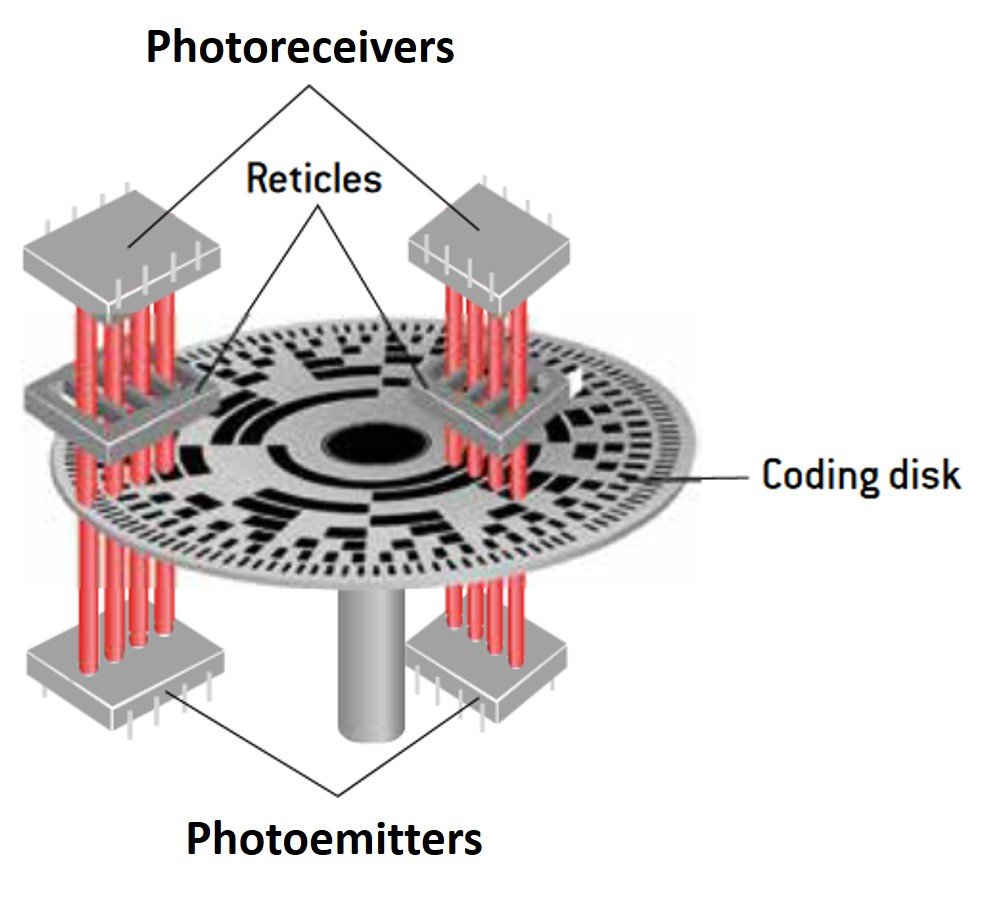
\includegraphics[width=0.7\linewidth]{Absolute-encoder}
%			\caption{}
			\label{fig:absolute-encoder}
		\end{figure}
		
		
	\end{flushleft}
\end{frame}



\begin{frame}{Binary vs gray code, 1}
	% \framesubtitle{O}
	\begin{flushleft}
		
		By its nature, the use of sensor implies that the signal will produce logical output of 0 or 1. This implies that encoding the orientation will be "binary-like".  
		
		\bigskip
		
		There are two popular types of encoding - binary code and gray code. 
		
	\end{flushleft}
\end{frame}




\begin{frame}{Binary vs gray code, 2}
	% \framesubtitle{O}
	\begin{flushleft}
		
		\begin{table}[]
			\begin{tabular}{lll}
				\textbf{Decimal} & \textbf{Binary} & \textbf{Gray} \\
				0       & 0000   & 0000 \\
				1       & 0001   & 0001 \\
				2       & 0010   & 0011 \\
				3       & 0011   & 0010 \\
				4       & 0100   & 0110 \\
				5       & 0101   & 0111 \\
				6       & 0110   & 0101 \\
				7       & 0111   & 0100 \\
				8       & 1000   & 1100 \\
				9       & 1001   & 1101 \\
				10      & 1010   & 1111 \\
				11      & 1011   & 1110 \\
				12      & 1100   & 1010 \\
				13      & 1101   & 1011 \\
				14      & 1110   & 1001 \\
				15      & 1111   & 1000
			\end{tabular}
		\end{table}
		
	\end{flushleft}
\end{frame}


\begin{frame}{Binary vs gray code, 3}
	% \framesubtitle{O}
	\begin{flushleft}
		
		We can notice that binary code changes multiple digits during a single increment. While gray code changes a single digits per increment.
		
		\bigskip
		
		The disadvantage changing multiple digits is the ambiguity during the transition. If even 2 digits simultaneously change during the transition, it means that there are at least 4 possible readings, only two of which are neighboring the current sensor position.
		
	\end{flushleft}
\end{frame}



\begin{frame}{Placement of optical sensors}
	% \framesubtitle{O}
	\begin{flushleft}
		
		Optical sensors can measure orientation of any shaft - including internal motor shaft and output gear box shaft. One of the ways to place such sensors is - place incremental encoder on the internal motor shaft, and absolute encoder on the output gear box shaft.
		
		\bigskip
		
		Internal motor shaft is rotating at higher angular velocity, providing more readings for the incremental encoder. This is especially useful in estimating angular velocity of the motor. However, backlash can make measurement of orientation with such an encoder dubious. Note that for velocity measurement absolute encoder does not hold an advantage over incremental one, and the latter is simpler in both design and signal processing.
		
		\bigskip
		
		Placing absolute encoder at the external shaft allows precise measurement of position, negating backlash. 
		
	\end{flushleft}
\end{frame}


\myqrframe

\end{document}
